\documentclass[
  shownotes,
  xcolor={svgnames},
  hyperref={colorlinks,citecolor=DarkBlue,linkcolor=DarkRed,urlcolor=DarkBlue}
  , aspectratio=169]{beamer}
\usepackage{animate}
\usepackage{amsmath}
\usepackage{amsfonts}
\usepackage{amssymb}
\usepackage{pifont}
\usepackage{mathpazo}
%\usepackage{xcolor}
\usepackage{multimedia}
\usepackage{fancybox}
\usepackage[para]{threeparttable}
\usepackage{multirow}
\setcounter{MaxMatrixCols}{30}
\usepackage{subcaption}
\usepackage{graphicx}
\usepackage{lscape}
\usepackage[compatibility=false,font=small]{caption}
\usepackage{booktabs}
\usepackage{ragged2e}
\usepackage{chronosys}
\usepackage{appendixnumberbeamer}
\usepackage{animate}
\setbeamertemplate{caption}[numbered]
\usepackage{color}
%\usepackage{times}
\usepackage{tikz}
\usepackage{comment} %to comment
%% BibTeX settings
\usepackage{natbib}
\bibliographystyle{apalike}
\bibpunct{(}{)}{,}{a}{,}{,}
\setbeamertemplate{bibliography item}{[\theenumiv]}

% Defines columns for bespoke tables
\usepackage{array}
\newcolumntype{L}[1]{>{\raggedright\let\newline\\\arraybackslash\hspace{0pt}}m{#1}}
\newcolumntype{C}[1]{>{\centering\let\newline\\\arraybackslash\hspace{0pt}}m{#1}}
\newcolumntype{R}[1]{>{\raggedleft\let\newline\\\arraybackslash\hspace{0pt}}m{#1}}


\usepackage{xfrac}


\usepackage{multicol}
\setlength{\columnsep}{0.5cm}

% Theme and colors
\usetheme{Boadilla}

% I use steel blue and a custom color palette. This defines it.
\definecolor{andesred}{HTML}{af2433}

% Other options
\providecommand{\U}[1]{\protect\rule{.1in}{.1in}}
\usefonttheme{serif}
\setbeamertemplate{itemize items}[default]
\setbeamertemplate{enumerate items}[square]
\setbeamertemplate{section in toc}[circle]

\makeatletter

\definecolor{mybackground}{HTML}{82CAFA}
\definecolor{myforeground}{HTML}{0000A0}

\setbeamercolor{normal text}{fg=black,bg=white}
\setbeamercolor{alerted text}{fg=red}
\setbeamercolor{example text}{fg=black}

\setbeamercolor{background canvas}{fg=myforeground, bg=white}
\setbeamercolor{background}{fg=myforeground, bg=mybackground}

\setbeamercolor{palette primary}{fg=black, bg=gray!30!white}
\setbeamercolor{palette secondary}{fg=black, bg=gray!20!white}
\setbeamercolor{palette tertiary}{fg=white, bg=andesred}

\setbeamercolor{frametitle}{fg=andesred}
\setbeamercolor{title}{fg=andesred}
\setbeamercolor{block title}{fg=andesred}
\setbeamercolor{itemize item}{fg=andesred}
\setbeamercolor{itemize subitem}{fg=andesred}
\setbeamercolor{itemize subsubitem}{fg=andesred}
\setbeamercolor{enumerate item}{fg=andesred}
\setbeamercolor{item projected}{bg=gray!30!white,fg=andesred}
\setbeamercolor{enumerate subitem}{fg=andesred}
\setbeamercolor{section number projected}{bg=gray!30!white,fg=andesred}
\setbeamercolor{section in toc}{fg=andesred}
\setbeamercolor{caption name}{fg=andesred}
\setbeamercolor{button}{bg=gray!30!white,fg=andesred}


\usepackage{fancyvrb}
\newcommand{\VerbBar}{|}
\newcommand{\VERB}{\Verb[commandchars=\\\{\}]}
\DefineVerbatimEnvironment{Highlighting}{Verbatim}{commandchars=\\\{\}}
% Add ',fontsize=\small' for more characters per line
\usepackage{framed}
\definecolor{shadecolor}{RGB}{248,248,248}
\newenvironment{Shaded}{\begin{snugshade}}{\end{snugshade}}
\newcommand{\AlertTok}[1]{\textcolor[rgb]{0.94,0.16,0.16}{#1}}
\newcommand{\AnnotationTok}[1]{\textcolor[rgb]{0.56,0.35,0.01}{\textbf{\textit{#1}}}}
\newcommand{\AttributeTok}[1]{\textcolor[rgb]{0.77,0.63,0.00}{#1}}
\newcommand{\BaseNTok}[1]{\textcolor[rgb]{0.00,0.00,0.81}{#1}}
\newcommand{\BuiltInTok}[1]{#1}
\newcommand{\CharTok}[1]{\textcolor[rgb]{0.31,0.60,0.02}{#1}}
\newcommand{\CommentTok}[1]{\textcolor[rgb]{0.56,0.35,0.01}{\textit{#1}}}
\newcommand{\CommentVarTok}[1]{\textcolor[rgb]{0.56,0.35,0.01}{\textbf{\textit{#1}}}}
\newcommand{\ConstantTok}[1]{\textcolor[rgb]{0.00,0.00,0.00}{#1}}
\newcommand{\ControlFlowTok}[1]{\textcolor[rgb]{0.13,0.29,0.53}{\textbf{#1}}}
\newcommand{\DataTypeTok}[1]{\textcolor[rgb]{0.13,0.29,0.53}{#1}}
\newcommand{\DecValTok}[1]{\textcolor[rgb]{0.00,0.00,0.81}{#1}}
\newcommand{\DocumentationTok}[1]{\textcolor[rgb]{0.56,0.35,0.01}{\textbf{\textit{#1}}}}
\newcommand{\ErrorTok}[1]{\textcolor[rgb]{0.64,0.00,0.00}{\textbf{#1}}}
\newcommand{\ExtensionTok}[1]{#1}
\newcommand{\FloatTok}[1]{\textcolor[rgb]{0.00,0.00,0.81}{#1}}
\newcommand{\FunctionTok}[1]{\textcolor[rgb]{0.00,0.00,0.00}{#1}}
\newcommand{\ImportTok}[1]{#1}
\newcommand{\InformationTok}[1]{\textcolor[rgb]{0.56,0.35,0.01}{\textbf{\textit{#1}}}}
\newcommand{\KeywordTok}[1]{\textcolor[rgb]{0.13,0.29,0.53}{\textbf{#1}}}
\newcommand{\NormalTok}[1]{#1}
\newcommand{\OperatorTok}[1]{\textcolor[rgb]{0.81,0.36,0.00}{\textbf{#1}}}
\newcommand{\OtherTok}[1]{\textcolor[rgb]{0.56,0.35,0.01}{#1}}
\newcommand{\PreprocessorTok}[1]{\textcolor[rgb]{0.56,0.35,0.01}{\textit{#1}}}
\newcommand{\RegionMarkerTok}[1]{#1}
\newcommand{\SpecialCharTok}[1]{\textcolor[rgb]{0.00,0.00,0.00}{#1}}
\newcommand{\SpecialStringTok}[1]{\textcolor[rgb]{0.31,0.60,0.02}{#1}}
\newcommand{\StringTok}[1]{\textcolor[rgb]{0.31,0.60,0.02}{#1}}
\newcommand{\VariableTok}[1]{\textcolor[rgb]{0.00,0.00,0.00}{#1}}
\newcommand{\VerbatimStringTok}[1]{\textcolor[rgb]{0.31,0.60,0.02}{#1}}
\newcommand{\WarningTok}[1]{\textcolor[rgb]{0.56,0.35,0.01}{\textbf{\textit{#1}}}}
\usepackage{graphicx}
\makeatletter


% colors
\definecolor{airforceblue}{rgb}{0.36, 0.54, 0.66}
\newcommand{\theme}{\color{andesred}}
\newcommand{\bk}{\color{black}}
\newcommand{\rd}{\color{red}}
\newcommand{\fg}{\color{ForestGreen}}
\newcommand{\bl}{\color{blue}}
\newcommand{\gr}{\color{black!60}}
\newcommand{\sg}{\color{DarkSlateGray}}
\newcommand{\br}{\color{SaddleBrown}}
\newcommand{\nv}{\color{Navy}}


% common math markups
\newcommand{\bs}[1]{\boldsymbol{#1}}
\newcommand{\mc}[1]{\mathcal{#1}}
\newcommand{\mr}[1]{\mathrm{#1}}
\newcommand{\bm}[1]{\mathbf{#1}}
\newcommand{\ds}[1]{\mathds{#1}}
\newcommand{\indep}{\perp\!\!\!\perp}



% shorthand
\newcommand{\sk}{\vspace{.5cm}}
\newcommand{\R}[1]{{\tt \nv #1}}
\newcommand{\til}{{\footnotesize$\bs{\stackrel{\sim}{}}$}}
\DeclareSymbolFont{extraup}{U}{zavm}{m}{n}
\DeclareMathSymbol{\vardiamond}{\mathalpha}{extraup}{87}

\usepackage{tikz}
% Tikz settings optimized for causal graphs.
\usetikzlibrary{shapes,decorations,arrows,calc,arrows.meta,fit,positioning}
\tikzset{
    -Latex,auto,node distance =1 cm and 1 cm,semithick,
    state/.style ={ellipse, draw, minimum width = 0.7 cm},
    point/.style = {circle, draw, inner sep=0.04cm,fill,node contents={}},
    bidirected/.style={Latex-Latex,dashed},
    el/.style = {inner sep=2pt, align=left, sloped}
}


\makeatother





%%%%%%%%%%%%%%% BEGINS DOCUMENT %%%%%%%%%%%%%%%%%%

\begin{document}

\title[Lecture 29]{Lecture 29: \\ Multinomial Logit \& Intro to Deep Learning }
\subtitle{Big Data and Machine Learning for Applied Economics \\ Econ 4676}
\date{\today}

\author[Sarmiento-Barbieri]{Ignacio Sarmiento-Barbieri}
\institute[Uniandes]{Universidad de los Andes}


\begin{frame}[noframenumbering]
\maketitle
\end{frame}

%%%%%%%%%%%%%%%%%%%%%%%%%%%%%%%%%%%


%%%%%%%%%%%%%%%%%%%%%%%%%%%%%%%%%%%


%----------------------------------------------------------------------%
\begin{frame}
\frametitle{Announcements }


\begin{itemize} 
    \item  Thursday turn in your predictions
    \bigskip
    \item  Friday PS5 and PS6 are due
    \bigskip
    \item  Next week presentations
    \bigskip
    
    
\end{itemize}
\end{frame}

%----------------------------------------------------------------------% 
\begin{frame}
\frametitle{Recap: Text as Data}

\begin{itemize} 
  
\item Topic Models
\bigskip
\item PCA Theory
\bigskip
\item Latent Dirichlet Allocation (LDA): Example
\bigskip
\item  Word Embedings
\end{itemize}
  
\end{frame}

%----------------------------------------------------------------------% 

\begin{frame}
\frametitle{Agenda}

\tableofcontents

\end{frame}

%----------------------------------------------------------------------%
\section{Multinomial Logit}
%----------------------------------------------------------------------%

\begin{frame}[fragile]
\frametitle{The multinomial logit model: Intuition}

\begin{itemize}
 \item We've seen different techniques to use text in a regression
 \medskip
 \item So far all have been linear models,
 \medskip
 \item But what happens when we have to predict multiple outcomes 
\end{itemize}





\end{frame}
%----------------------------------------------------------------------%
\begin{frame}[fragile]
\frametitle{The multinomial logit model: Intuition}



\begin{itemize}
 \item The MNLM can be thought of as simultaneously fitting binary logits for all comparisons among the alternatives. 
\medskip
 \item For example, 
 \medskip
\begin{itemize}
    \item We have  a categorical variable with the outcomes for Democrat, for Independent, and for Republican.
      \medskip
    \item Assume that there is one independent variable measuring income in $1,000s$. 
      \medskip
    \item We can examine the effect of income on party by fitting three binary logits,
\end{itemize}
 

\end{itemize}

\end{frame}
%----------------------------------------------------------------------%
\begin{frame}[fragile]
\frametitle{The multinomial logit model: Intuition}



\begin{itemize}
 \item The MNLM can be thought of as simultaneously fitting binary logits for all comparisons among the alternatives. 
\medskip
  \begin{align}
  \ln \frac{Pr(D|X)}{Pr(I/X)}=\beta_{0,D|I} +\beta_{1,D|I} Income \\ \nonumber
  \ln \frac{Pr(R|X)}{Pr(I/X)}=\beta_{0,R|I} +\beta_{1,R|I} Income \\ \nonumber
  \ln \frac{Pr(D|X)}{Pr(R/X)}=\beta_{0,D|R} +\beta_{1,D|R} Income \\ \nonumber
  \end{align}

\item where the subscripts to the $\beta's$ indicate which comparison is being made. 



\end{itemize}


\end{frame}
%----------------------------------------------------------------------%
\begin{frame}[fragile]
\frametitle{The multinomial logit model: Intuition}



\begin{itemize}
 \item These logits include redundant info
\medskip
\begin{align}
\ln \frac{Pr(D|X)}{Pr(I/X)}- \ln \frac{Pr(R|X)}{Pr(I/X)}= \ln \frac{Pr(D|X)}{Pr(R/X)}
\end{align}

\medskip
\item which implies
\medskip
 \begin{align}
  \beta_{0,D|I} - \beta_{0,R|I} &=\beta_{0,D|R} \\
  \beta_{1,D|I}-\beta_{1,R|I} &= \beta_{1,D|R} 
\end{align}

\medskip
\item In general, with $J$ alternatives, only $J-1$ binary logits need to be fit (minimal set)

 

\end{itemize}

\end{frame}
%----------------------------------------------------------------------%
\begin{frame}[fragile]
\frametitle{The multinomial logit model: Intuition}




\begin{table}[H]
\scriptsize
\begin{tabular}{lcccccc} \hline
&\multicolumn{3}{c}{Binary} & \multicolumn{3}{c}{Multinomial Logit} \\
 & (1) & (2) & (3) & & & \\
VARIABLES & dem\_ind & rep\_ind & dem\_rep & Democrat & Independent & Republican \\ \hline
 &  &  &  &  &  &  \\
income & -0.00249 & 0.0157*** & -0.0184*** & -0.00272 &  & 0.0152*** \\
 & (0.00355) & (0.00374) & (0.00230) & (0.00372) &  & (0.00366) \\
Constant & 1.605*** & 0.659*** & 0.953*** & 1.613*** &  & 0.678*** \\
 & (0.149) & (0.162) & (0.105) & (0.153) &  & (0.160) \\
 &  &  &  &  &  &  \\
 Observations & 844 & 689 & 1,231 & 1,382 & 1,382 & 1,382 \\ \hline

\end{tabular}
\end{table}



\begin{itemize}
 \item Fitting the MNLM by fitting a series of binary logits is not optimal
 \medskip
   \begin{itemize}
   \item  Binary logit is based on a different sample. 
   \medskip
  \item It ignores the restricctions that are implicit in the definition of the MNLM
  \end{itemize}
\end{itemize}



\end{frame}
%----------------------------------------------------------------------%
\begin{frame}[fragile]
\frametitle{The multinomial logit model: formal statement}

\begin{itemize}
\item Formally
\medskip 
\begin{align}
\ln \Omega_{m|b}(X)=\ln \frac{Pr(y=m|X)}{Pr(y=b|X)}=X\beta_{m|b} \,\,\, for\, m=1, \dots, J
\end{align}
\medskip 
\item were $b$ is the base outcome (reference category)
\medskip 
\item These J equations can be solved to compute the probabilities for each outcome
\end{itemize}

  \begin{align}
  Pr(y=m|X) = \frac{exp(X\beta_{m|b})}{\sum_{j=1}^J exp(X\beta_{j|b})}
  \end{align}

\end{frame}
%----------------------------------------------------------------------%
\subsection{Multinomial Inverse Regression}
%----------------------------------------------------------------------%
\begin{frame}
\frametitle{Multinomial Inverse Regression}


\begin{itemize}

  \item A task that comes up often in social science is understanding how text connects to a set of related covariates. 
  \medskip
  \item For example, you might want to connect the \texttt{we8there} reviews simultaneously to all five aspect ratings, allowing you to determine which content is predictive of ratings on, say, atmosphere separate from food or service. 
  \medskip
  \item  For such tasks, we can turn to multinomial inverse regression (MNIR) to link the text with observable covariates through a multinomial distribution. 
\end{itemize}

\end{frame}
%----------------------------------------------------------------------%
\begin{frame}
\frametitle{Multinomial Inverse Regression}


\begin{itemize}
  \item The  ``inverse'' in MNIR comes from the fact that, while text regression usually fits a single document attribute as a function of word counts, we are inverting the process by regressing the counts on any number of document attributes. 
  \medskip
  \item Given document attributes $v_i$ (author characteristics, date, beliefs, sentiment, etc.), MNIR follows the familiar generalized linear model framework. 
  \medskip
  \item Each document $x_i$ is modeled as arising from a multinomial with a logit link onto a linear function of $v_i$
\end{itemize}

\end{frame}
%----------------------------------------------------------------------%
\begin{frame}
\frametitle{Multinomial Inverse Regression}

\begin{itemize}
\item Each document $x_i$ is modeled as arising from a multinomial with a logit link onto a linear function of $v_i$
\medskip
\begin{align}
x_i \sim MN(q_i,m_i)
\end{align}

\item with


\begin{align}
q_{ij}=\frac{exp(\alpha_j + v_i'\phi_j)}{\sum_{l=1}^p exp(\alpha_l + v_i'\phi_l)}
\end{align}
\medskip

\item Now, the number of outcome categories is the number of tokens in our text vocabulary. This can be viewed as a natural extension of topic modeling: we are keeping the multinomial model for token counts but replacing unknown topics with known attributes.
\end{itemize}



\end{frame}


%----------------------------------------------------------------------%
\begin{frame}
\frametitle{Multinomial Inverse Regression: Example}

\begin{itemize}


\item We have 6,166 reviews, with an average length of 90 words per review, \url{we8there.com}. 
\medskip
\item A useful feature of these reviews is that they contain both text and a multidimensional rating on overall experience, atmosphere, food, service, and value. 
\medskip
\item For example, one user submitted a glowing review for Waffle House \#1258 in Bossier City, Louisiana: 
\medskip

\begin{quote}
I normally would not revue a Waffle House but this one deserves it. The workers, Amanda, Amy, Cherry, James and J.D. were the most pleasant crew I have seen. While it was only lunch, B.L.T. and chili, it was great. The best thing was the 50’ s rock and roll music, not to loud not to soft. This is a rare exception to what you all think a Waffle House is. Keep up the good work. \\
Overall: 5, Atmosphere: 5, Food: 5, Service: 5, Value: 5.  
 \end{quote} 


\end{itemize}





\end{frame}

%----------------------------------------------------------------------%
\begin{frame}
\frametitle{Multinomial Inverse Regression: Example}

\begin{itemize}
\item Looking again at the  \texttt{we8there} data, we can set $v_i$ as the vector of five aspect ratings: 

\begin{enumerate}
  \item overall
  \item atmosphere
  \item value
  \item food 
  \item service
\end{enumerate}
\medskip
\item The multinomial response will be the vector of word counts for each review $x_i$, which implies 2640 outcome categories.

  \end{itemize}



\end{frame}

%----------------------------------------------------------------------%
\begin{frame}
\frametitle{Multinomial Inverse Regression: Example}

\begin{figure}[H] \centering
            \captionsetup{justification=centering}
              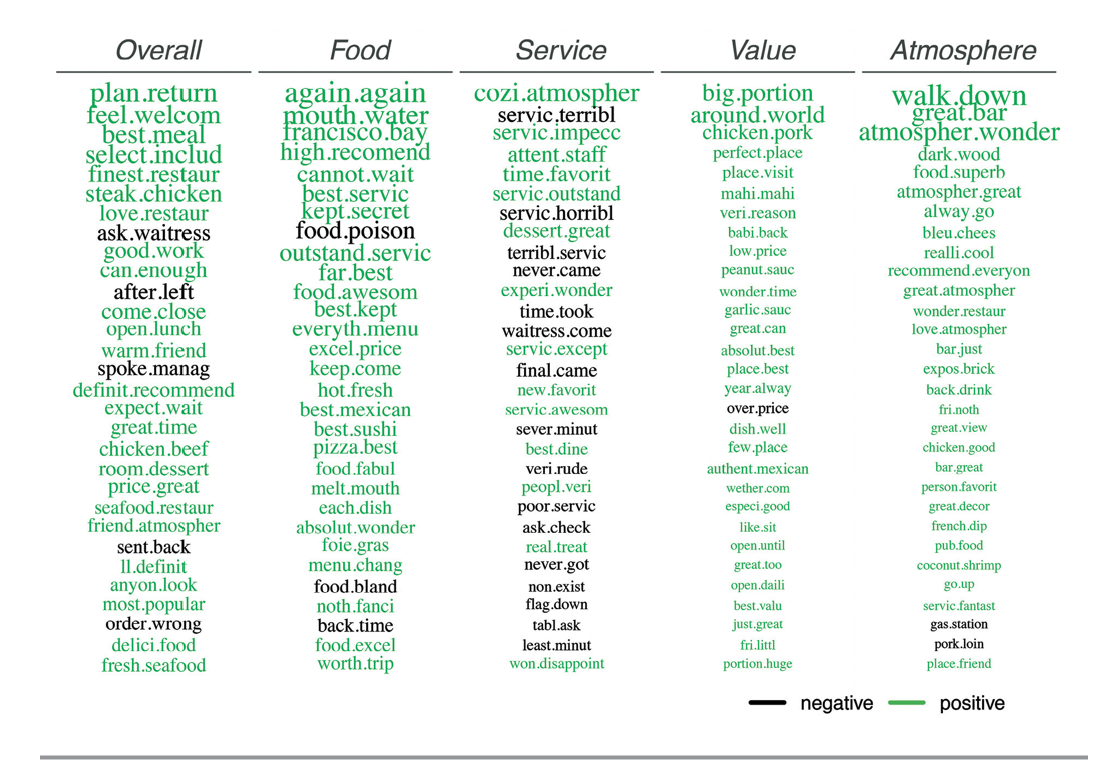
\includegraphics[scale=0.5]{figures/MNIR_regression.png}
              
 \end{figure}

\end{frame}

%----------------------------------------------------------------------%
\begin{frame}
\frametitle{Multinomial Inverse Regression: Example}
\begin{itemize}
\item This is truly a Big Data problem
\medskip
\item Traditional multiomial packages won't work
\medskip
\item In \texttt{R} you can use the package \texttt{distrom} 
\medskip
\item It was designed to be efficient for these types of massive-response multinomials. 
\medskip
\item It uses a Poisson distribution representation of the multinomial to distribute computation for each vocabulary element across multiple processors.

\end{itemize}
\end{frame}
%----------------------------------------------------------------------%
\section{Deep Learning: Intro}
%----------------------------------------------------------------------%
\begin{frame}
\frametitle{Deep Learning: Intro}
\pause
\begin{itemize}
    
  \item Neural networks are simple models.
  \medskip
  \item Their strength lays in their simplicity because basic patterns facilitate fast training and computation. 
  \medskip
  \item The model has linear combinations of inputs that are passed through nonlinear activation functions called nodes (or, in reference to the human brain, neurons). 
  \medskip
  
\end{itemize}

\end{frame}
%----------------------------------------------------------------------%
\begin{frame}
\frametitle{Deep Learning: Intro}
  
  
  \begin{itemize}
    \item Let's start with a familiar and simple model, the linear model
  
  \end{itemize}

\def\layersep{2.5cm}

\begin{align}
y &= f(X) + u \\ \nonumber
y &= \beta_1 x_1 + \beta_2 x_2 + \beta_3 x_3  + u
\end{align}
\pause

\begin{figure}[H]
\centering

\begin{tikzpicture}[shorten >=1pt,->,draw=black!50, node distance=\layersep]
    \tikzstyle{every pin edge}=[<-,shorten <=1pt]
    \tikzstyle{neuron}=[circle,fill=black!25,minimum size=17pt,inner sep=0pt]
    \tikzstyle{input neuron}=[neuron, fill=green!50];
    \tikzstyle{output neuron}=[neuron, fill=red!50];
    \tikzstyle{annot} = [text width=4em, text centered]

    % Draw the input layer nodes
    \foreach \name / \y in {1,...,3}
    % This is the same as writing \foreach \name / \y in {1/1,2/2,3/3,4/4}
        \node[input neuron, pin=left:$x_\y$] (I-\name) at (0,-\y) {};

    % Draw the output layer node
    \node[output neuron,pin={[pin edge={->}]right:y}, right of=I-2] (O) {};

    % Connect every node in the input layer with every node in the
    % hidden layer.
    

    % Connect every node in the hidden layer with the output layer
    \foreach \source in {1,...,3}
        \path (I-\source) edge (O);

    \node[annot,above of=I-1, node distance=1cm] (i) {Input layer};
    \node[annot,right of=i] {Output layer};

\end{tikzpicture}
\end{figure}



\end{frame}
%----------------------------------------------------------------------%
\begin{frame}
\frametitle{Multilayer Perceptrons}

\begin{itemize}
    \item Linear Models may be to simple, and miss the nonlinearities that best approximate $f^*(x)$
    \medskip
    \item We can overcome these limitations of linear models and handle a more general class of functions by incorporating one or more hidden layers.
    \medskip
    \item Deep feed forward networks, also called feed forward neural networks, or multilayer perceptrons (MLPs), are the quintessential deep learning models
\end{itemize}

\end{frame}
%----------------------------------------------------------------------%
\begin{frame}
\frametitle{Multilayer Perceptrons}

\begin{itemize}

\item Feed forward neural networks are called networks because they are typically represented by composing together many different functions. 
\medskip
\item For example, we might have two functions $f^{(2)}$, $f^{(1)}$ and connected in a chain to form $f(x)=f^{(2)}(f^{(1)}(x))$ 
\medskip
 \item These chain structures are the most commonly used structures of neural networks. 
\end{itemize}
\end{frame}

%----------------------------------------------------------------------%
\begin{frame}
\frametitle{Multilayer Perceptrons}


\def\layersep{2.5cm}

\begin{figure}[H]
\centering
\begin{tikzpicture}[shorten >=1pt,->,draw=black!50, node distance=\layersep]
    \tikzstyle{every pin edge}=[<-,shorten <=1pt]
    \tikzstyle{neuron}=[circle,fill=black!25,minimum size=17pt,inner sep=0pt]
    \tikzstyle{input neuron}=[neuron, fill=green!50];
    \tikzstyle{output neuron}=[neuron, fill=red!50];
    \tikzstyle{hidden neuron}=[neuron, fill=blue!50];
    \tikzstyle{annot} = [text width=4em, text centered]

    % Draw the input layer nodes
    \foreach \name / \y in {1,...,4}
    % This is the same as writing \foreach \name / \y in {1/1,2/2,3/3,4/4}
        \node[input neuron, pin=left: $x_\y$] (I-\name) at (0,-\y) {};

    % Draw the hidden layer nodes
    \foreach \name / \y in {1,...,5}
        \path[yshift=0.5cm]
            node[hidden neuron] (H-\name) at (\layersep,-\y cm) {};

    % Draw the output layer node
    \node[output neuron,pin={[pin edge={->}]right:y}, right of=H-3] (O) {};

    % Connect every node in the input layer with every node in the
    % hidden layer.
    \foreach \source in {1,...,4}
        \foreach \dest in {1,...,5}
            \path (I-\source) edge (H-\dest);

    % Connect every node in the hidden layer with the output layer
    \foreach \source in {1,...,5}
        \path (H-\source) edge (O);

    % Annotate the layers
    \node[annot,above of=H-1, node distance=1cm] (hl) {Hidden layer};
    \node[annot,left of=hl] {Input layer};
    \node[annot,right of=hl] {Output layer};
\end{tikzpicture}
\end{figure}

\end{frame}
%----------------------------------------------------------------------%
\begin{frame}
\frametitle{Multilayer Perceptrons}


\begin{itemize}



\item The overall length of the chain gives the depth of the model. The name “deep learning” arose from this terminology. 
\medskip 
\item The final layer of a feed forward network is called the output layer
\medskip
\item During neural network training, we try to train $f(x)$ to match $f^*(x)$
\medskip
\item In the training data we observe the first layer, inputs ($x$), and the last layer, output ($y$)
\medskip
\item We do not observe the intermediate layers,they are then called hidden layers.
\medskip
\item Finally, these networks are called neural because they are loosely inspired by
neuroscience.



\end{itemize}
\end{frame}

%----------------------------------------------------------------------%
\begin{frame}[fragile]
\frametitle{Deep Learning: Demo}





\begin{Shaded}
\begin{Highlighting}[]
\KeywordTok{library}\NormalTok{(keras)}
\NormalTok{fashion\_mnist \textless{}{-}}\StringTok{ }\KeywordTok{dataset\_fashion\_mnist}\NormalTok{()}
\end{Highlighting}
\end{Shaded}

  \begin{figure}[H] \centering
            \captionsetup{justification=centering}
              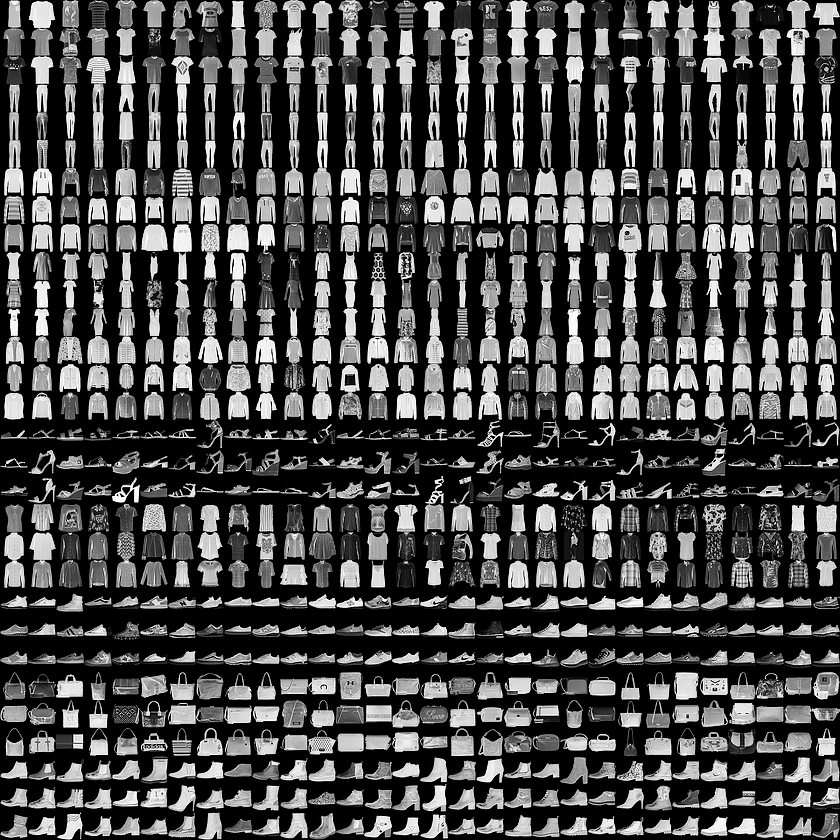
\includegraphics[scale=0.4]{figures/fashion-mnist-sprite}
              
 \end{figure}
\end{frame}
% %----------------------------------------------------------------------%
\begin{frame}[fragile]
\frametitle{Deep Learning: Demo}
  \begin{figure}[H] \centering
            \captionsetup{justification=centering}
              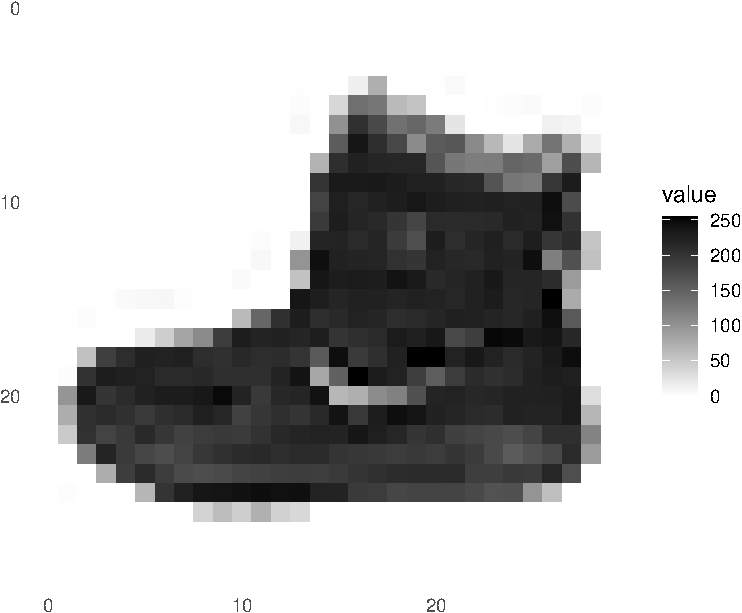
\includegraphics[scale=0.4]{figures/unnamed-chunk-3-1.pdf}
              
 \end{figure}


\end{frame}
%----------------------------------------------------------------------%
\begin{frame}[fragile]
\frametitle{Deep Learning: Demo}

\begin{Shaded}
\begin{Highlighting}[]
\NormalTok{train\_images \textless{}{-}}\StringTok{ }\NormalTok{train\_images }\OperatorTok{/}\StringTok{ }\DecValTok{255}
\NormalTok{test\_images \textless{}{-}}\StringTok{ }\NormalTok{test\_images }\OperatorTok{/}\StringTok{ }\DecValTok{255}
\end{Highlighting}
\end{Shaded}



\begin{Shaded}
\begin{Highlighting}[]
\NormalTok{model \textless{}{-}}\StringTok{ }\KeywordTok{keras\_model\_sequential}\NormalTok{()}
\NormalTok{model }\OperatorTok{\%\textgreater{}\%}
\StringTok{  }\KeywordTok{layer\_flatten}\NormalTok{(}\DataTypeTok{input\_shape =} \KeywordTok{c}\NormalTok{(}\DecValTok{28}\NormalTok{, }\DecValTok{28}\NormalTok{)) }\OperatorTok{\%\textgreater{}\%}
\StringTok{  }\KeywordTok{layer\_dense}\NormalTok{(}\DataTypeTok{units =} \DecValTok{128}\NormalTok{, }\DataTypeTok{activation =} \StringTok{\textquotesingle{}relu\textquotesingle{}}\NormalTok{) }\OperatorTok{\%\textgreater{}\%}
\StringTok{  }\KeywordTok{layer\_dense}\NormalTok{(}\DataTypeTok{units =} \DecValTok{10}\NormalTok{, }\DataTypeTok{activation =} \StringTok{\textquotesingle{}softmax\textquotesingle{}}\NormalTok{)}
\end{Highlighting}
\end{Shaded}

\begin{Shaded}
\begin{Highlighting}[]
\NormalTok{model }\OperatorTok{\%\textgreater{}\%}\StringTok{ }\KeywordTok{compile}\NormalTok{(}
  \DataTypeTok{optimizer =} \StringTok{\textquotesingle{}adam\textquotesingle{}}\NormalTok{, }
  \DataTypeTok{loss =} \StringTok{\textquotesingle{}sparse\_categorical\_crossentropy\textquotesingle{}}\NormalTok{,}
  \DataTypeTok{metrics =} \KeywordTok{c}\NormalTok{(}\StringTok{\textquotesingle{}accuracy\textquotesingle{}}\NormalTok{)}
\NormalTok{)}
\NormalTok{model }\OperatorTok{\%\textgreater{}\%}\StringTok{ }\KeywordTok{fit}\NormalTok{(train\_images, train\_labels, }\DataTypeTok{epochs =} \DecValTok{5}\NormalTok{, }\DataTypeTok{verbose =} \DecValTok{2}\NormalTok{)}
\end{Highlighting}
\end{Shaded}

\end{frame}
%----------------------------------------------------------------------%
\begin{frame}[fragile]
\frametitle{Deep Learning: Demo}
\begin{scriptsize}
\begin{verbatim}
## Epoch 1/5
## 1875/1875 - 2s - loss: 0.5003 - accuracy: 0.8238
## Epoch 2/5
## 1875/1875 - 2s - loss: 0.3782 - accuracy: 0.8643
## Epoch 3/5
## 1875/1875 - 2s - loss: 0.3362 - accuracy: 0.8784
## Epoch 4/5
## 1875/1875 - 2s - loss: 0.3141 - accuracy: 0.8844
## Epoch 5/5
## 1875/1875 - 2s - loss: 0.2934 - accuracy: 0.8922
\end{verbatim}
\end{scriptsize}

\begin{Shaded}
\begin{Highlighting}[]
\NormalTok{score \textless{}{-}}\StringTok{ }\NormalTok{model }\OperatorTok{\%\textgreater{}\%}\StringTok{ }\KeywordTok{evaluate}\NormalTok{(test\_images, test\_labels, }\DataTypeTok{verbose =} \DecValTok{0}\NormalTok{)}

\KeywordTok{cat}\NormalTok{(}\StringTok{\textquotesingle{}Test loss:\textquotesingle{}}\NormalTok{, score[}\DecValTok{1}\NormalTok{], }\StringTok{"}\CharTok{\textbackslash{}n}\StringTok{"}\NormalTok{)}
\end{Highlighting}
\end{Shaded}
\begin{scriptsize}

\begin{verbatim}
## Test loss: 0.3377942

## Test accuracy: 0.8792
\end{verbatim}
\end{scriptsize}
\end{frame}

%----------------------------------------------------------------------%
\section{Word Embedding: Demo }
%----------------------------------------------------------------------%
\begin{frame}[fragile]
\frametitle{Word Embedding: Demo }
\pause
\begin{itemize}
  \item In the original deep learning context, embedding layers replace each word with a vector value
  \begin{itemize}
    \item for example, man becomes the location [1,2, 0.25] in a three-dimensional embedding space% (this is just for illustration; embedding spaces are typically of more than 100 dimensions). 
   
\end{itemize} 
  \begin{figure}[H] \centering
            \captionsetup{justification=centering}
              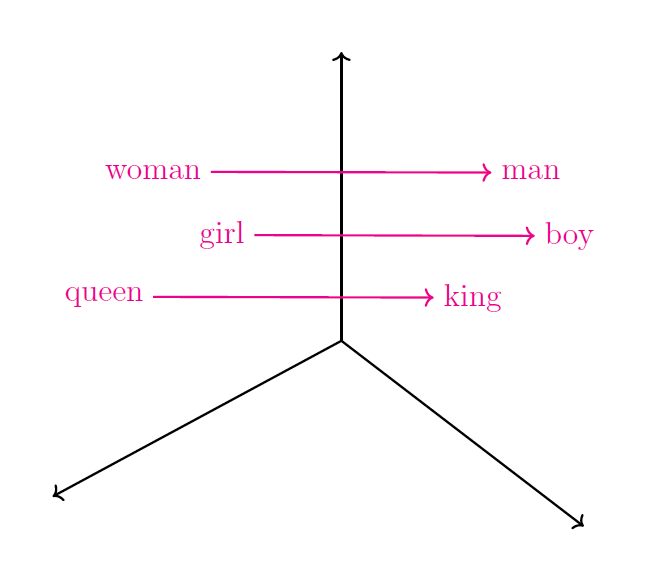
\includegraphics[scale=0.4]{figures/embedings.png}
              
 \end{figure}

 \item Word embeddings preserve semantic relationships.
  \begin{itemize}
    \item Words with similar meaning have similar representations.
    \medskip
    \item Dimensions induced by word differences can be used to identify cultural concepts 
  \end{itemize}
  \end{itemize} 
\end{frame}


%----------------------------------------------------------------------%
\begin{frame}[fragile]
\frametitle{Word Embedding: Demo }

\begin{itemize}
  \item  The dimensions are useful because they produce quantitative measures of similarity between the associated concepts and specific words in the corpus. 
  \end{itemize}

   \begin{figure}[H] \centering
            \captionsetup{justification=centering}
              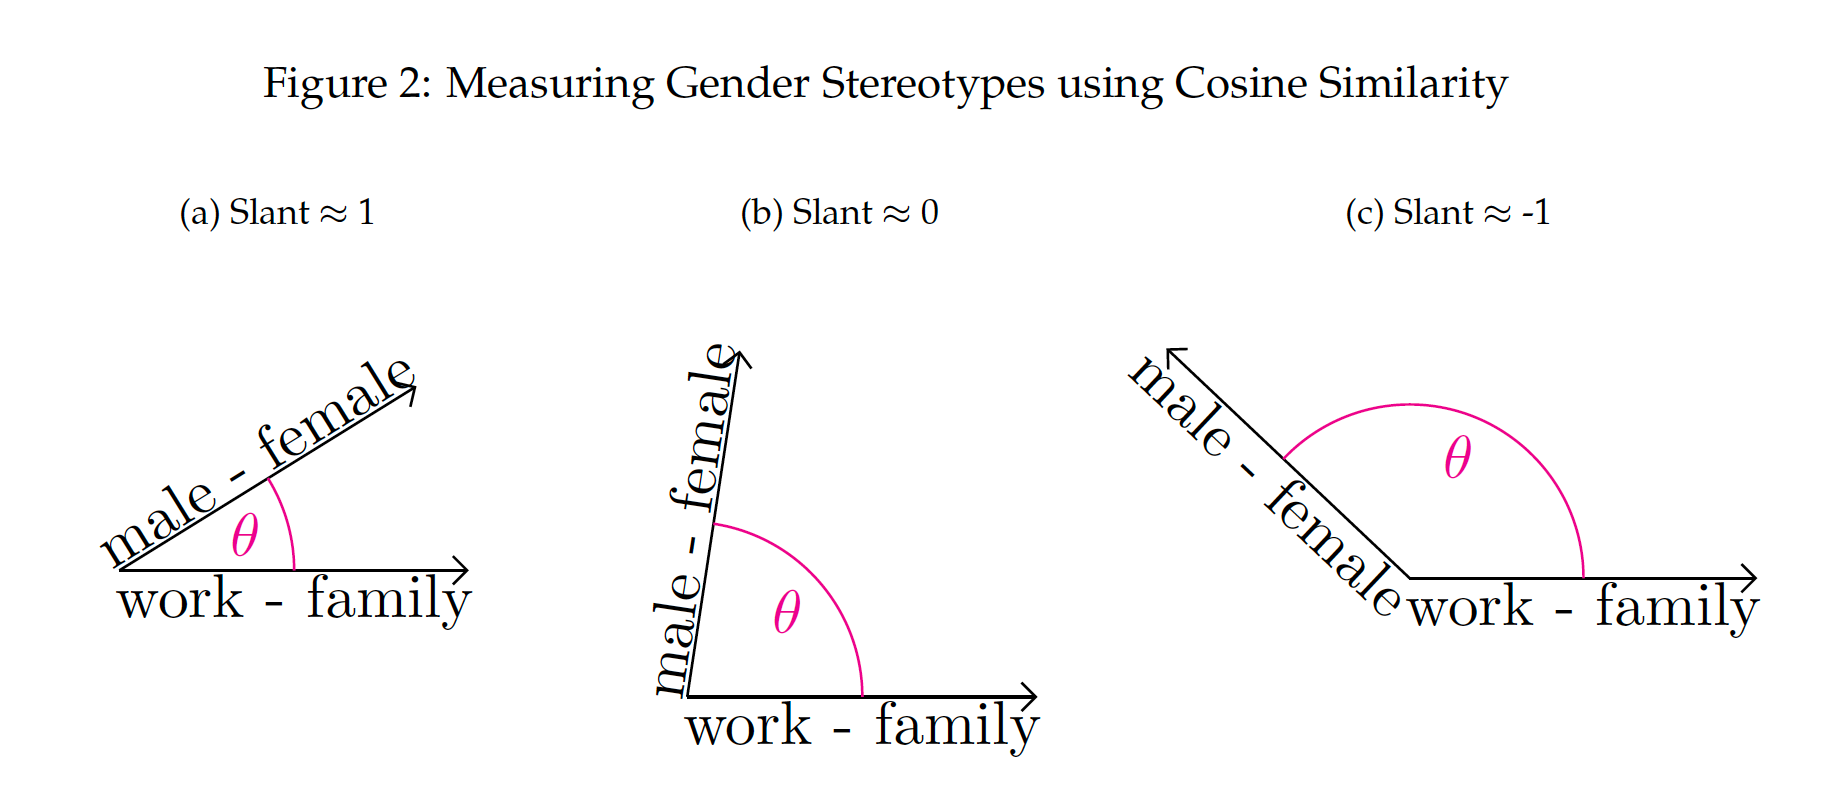
\includegraphics[scale=0.4]{figures/gender_slant.png}
              
 \end{figure}
\end{frame}
%----------------------------------------------------------------------%
\begin{frame}[fragile]
\frametitle{Word Embedding: Demo }

\begin{scriptsize}
\begin{Shaded}
\begin{Highlighting}[]
\KeywordTok{library}\NormalTok{(text2vec)}
\KeywordTok{load}\NormalTok{(}\StringTok{\textquotesingle{}shakes\_words\_df\_4text2vec.RData\textquotesingle{}}\NormalTok{)}
\KeywordTok{head}\NormalTok{(shakes\_words)}
\end{Highlighting}
\end{Shaded}

\end{scriptsize}
\begin{tiny}


\begin{verbatim}
##                    id         word
## 1 A_Lover_s_Complaint          nor
## 2 A_Lover_s_Complaint        gives
## 3 A_Lover_s_Complaint           it
## 4 A_Lover_s_Complaint satisfaction
## 5 A_Lover_s_Complaint           to
\end{verbatim}
\end{tiny}

\begin{scriptsize}

\begin{Shaded}
\begin{Highlighting}[]
\NormalTok{shakes\_words\_ls \textless{}{-}}\StringTok{ }\KeywordTok{list}\NormalTok{(shakes\_words}\OperatorTok{$}\NormalTok{word)}
\NormalTok{it \textless{}{-}}\StringTok{ }\KeywordTok{itoken}\NormalTok{(shakes\_words\_ls, }\DataTypeTok{progressbar =} \OtherTok{FALSE}\NormalTok{)}
\NormalTok{shakes\_vocab \textless{}{-}}\StringTok{ }\KeywordTok{create\_vocabulary}\NormalTok{(it)}
\NormalTok{shakes\_vocab \textless{}{-}}\StringTok{ }\KeywordTok{prune\_vocabulary}\NormalTok{(shakes\_vocab, }\DataTypeTok{term\_count\_min=} \DecValTok{5}\NormalTok{)}
\KeywordTok{head}\NormalTok{(shakes\_vocab)}
\end{Highlighting}
\end{Shaded}

\end{scriptsize}
\begin{tiny}


\begin{verbatim}
## Number of docs: 1 
## 0 stopwords:  ... 
## ngram_min = 1; ngram_max = 1 
## Vocabulary: 
##         term term_count doc_count
## 1:    abbess          5         1
## 2: abilities          5         1
## 3: accessary          5         1
## 4:       ace          5         1
## 5:    adders          5         1
\end{verbatim}
\end{tiny}

\end{frame}
%----------------------------------------------------------------------%
\begin{frame}[fragile]
\frametitle{Word Embedding: Demo }

\begin{itemize}
\item The next step is to create the token co-occurrence matrix (TCM). 
\item The definition of whether two words occur together is arbitrary. 
%\item Should we just look at previous and next word? Five behind and forward? This will definitely affect results so you will want to play around with it.
\end{itemize}

\begin{scriptsize}

\begin{Shaded}
\begin{Highlighting}[]
\CommentTok{\# maps words to indices}
\NormalTok{vectorizer \textless{}{-}}\StringTok{ }\KeywordTok{vocab\_vectorizer}\NormalTok{(shakes\_vocab)}

\CommentTok{\# use window of 10 for context words}
\NormalTok{shakes\_tcm \textless{}{-}}\StringTok{ }\KeywordTok{create\_tcm}\NormalTok{(it, vectorizer, }\DataTypeTok{skip\_grams\_window =} \DecValTok{10}\NormalTok{)}
\end{Highlighting}
\end{Shaded}
\end{scriptsize}



\begin{itemize}
\item Now we are ready to create the word vectors based on the GloVe model.
\end{itemize}


\begin{scriptsize}


\begin{Shaded}
\begin{Highlighting}[]
\NormalTok{glove \textless{}{-}}\StringTok{ }\NormalTok{GlobalVectors}\OperatorTok{$}\KeywordTok{new}\NormalTok{(}\DataTypeTok{rank =} \DecValTok{50}\NormalTok{, }\DataTypeTok{x\_max =} \DecValTok{10}\NormalTok{)}
\NormalTok{shakes\_wv\_main =}\StringTok{ }\NormalTok{glove}\OperatorTok{$}\KeywordTok{fit\_transform}\NormalTok{(shakes\_tcm, }\DataTypeTok{n\_iter =} \DecValTok{10}\NormalTok{, }\DataTypeTok{convergence\_tol =} \FloatTok{0.01}\NormalTok{, }\DataTypeTok{n\_threads =} \DecValTok{8}\NormalTok{)}
\end{Highlighting}
\end{Shaded}


\end{scriptsize}
\begin{tiny}


\begin{verbatim}
## INFO  [16:55:06.317] epoch 1, loss 0.1242 
## INFO  [16:55:08.764] epoch 2, loss 0.0844 
## INFO  [16:55:11.249] epoch 3, loss 0.0762 
## INFO  [16:55:13.680] epoch 4, loss 0.0707 
## INFO  [16:55:16.109] epoch 5, loss 0.0666 
## INFO  [16:55:18.540] epoch 6, loss 0.0634 
## INFO  [16:55:20.980] epoch 7, loss 0.0609 
## INFO  [16:55:23.419] epoch 8, loss 0.0589 
## INFO  [16:55:25.849] epoch 9, loss 0.0572 
## INFO  [16:55:28.288] epoch 10, loss 0.0558
\end{verbatim}
\end{tiny}
\end{frame}
%----------------------------------------------------------------------%
\begin{frame}[fragile]
\frametitle{Word Embedding: Demo }

\begin{scriptsize}

\begin{Shaded}
\begin{Highlighting}[]
\KeywordTok{dim}\NormalTok{(shakes\_wv\_main)}
\end{Highlighting}
\end{Shaded}
\end{scriptsize}
\begin{tiny}
\begin{verbatim}
## [1] 9094   50
\end{verbatim}
\end{tiny}

\begin{scriptsize}


\begin{Shaded}
\begin{Highlighting}[]
\NormalTok{shakes\_wv\_context \textless{}{-}}\StringTok{ }\NormalTok{glove}\OperatorTok{$}\NormalTok{components}

\KeywordTok{dim}\NormalTok{(shakes\_wv\_context)}
\end{Highlighting}
\end{Shaded}
\end{scriptsize}
\begin{tiny}

\begin{verbatim}
## [1]   50 9094
\end{verbatim}
\end{tiny}

\begin{scriptsize}


\begin{Shaded}
\begin{Highlighting}[]
\CommentTok{\# Either word{-}vectors matrices could work, but the developers of the technique}
\CommentTok{\# suggest the sum/mean may work better}
\NormalTok{shakes\_word\_vectors \textless{}{-}}\StringTok{ }\NormalTok{shakes\_wv\_main }\OperatorTok{+}\StringTok{ }\KeywordTok{t}\NormalTok{(shakes\_wv\_context)}

\NormalTok{rom \textless{}{-}}\StringTok{ }\NormalTok{shakes\_word\_vectors[}\StringTok{"romeo"}\NormalTok{, , drop =}\StringTok{ }\NormalTok{F]}

\NormalTok{cos\_sim\_rom \textless{}{-}}\StringTok{ }\KeywordTok{sim2}\NormalTok{(}\DataTypeTok{x =}\NormalTok{shakes\_word\_vectors, }\DataTypeTok{y =}\NormalTok{ rom, }\DataTypeTok{method =} \StringTok{"cosine"}\NormalTok{, }\DataTypeTok{norm =} \StringTok{"l2"}\NormalTok{)}
\CommentTok{\# head(sort(cos\_sim\_rom[,1], decreasing \textless{}{-} T), 10)}
\end{Highlighting}
\end{Shaded}

\end{scriptsize}
\begin{tiny}

\begin{verbatim}
##     romeo    juliet    tybalt     nurse  benvolio  banished  
## 1.0000000 0.7712391 0.7575977 0.6697068 0.6517349 0.6436404  
\end{verbatim}
\end{tiny}


\end{frame}

%----------------------------------------------------------------------%
\begin{frame}[fragile]
\frametitle{Word Embedding: Demo }

\begin{scriptsize}


\begin{Shaded}
\begin{Highlighting}[]
\NormalTok{test \textless{}{-}}\StringTok{ }\NormalTok{shakes\_word\_vectors[}\StringTok{"romeo"}\NormalTok{, , drop =}\StringTok{ }\NormalTok{F] }\OperatorTok{{-}}
\StringTok{  }\NormalTok{shakes\_word\_vectors[}\StringTok{"mercutio"}\NormalTok{, , drop =}\StringTok{ }\NormalTok{F] }\OperatorTok{+}
\StringTok{  }\NormalTok{shakes\_word\_vectors[}\StringTok{"nurse"}\NormalTok{, , drop =}\StringTok{ }\NormalTok{F]}

\NormalTok{cos\_sim\_test \textless{}{-}}\StringTok{ }\KeywordTok{sim2}\NormalTok{(}\DataTypeTok{x =}\NormalTok{ shakes\_word\_vectors, }\DataTypeTok{y =}\NormalTok{ test, }\DataTypeTok{method =} \StringTok{"cosine"}\NormalTok{, }\DataTypeTok{norm =} \StringTok{"l2"}\NormalTok{)}
\KeywordTok{head}\NormalTok{(}\KeywordTok{sort}\NormalTok{(cos\_sim\_test[,}\DecValTok{1}\NormalTok{], }\DataTypeTok{decreasing =}\NormalTok{ T), }\DecValTok{10}\NormalTok{)}
\end{Highlighting}
\end{Shaded}
\end{scriptsize}
\begin{tiny}


\begin{verbatim}
##     nurse    juliet     romeo      lady    mother       bed         o      wife 
## 0.8904362 0.7584004 0.7179267 0.6440354 0.6374490 0.5880860 0.5756074 0.5638571 
##   capulet    dromio 
## 0.5520459 0.5507196
\end{verbatim}
\end{tiny}



\end{frame}
%----------------------------------------------------------------------%
\section{Review
 \& Next Steps}
%----------------------------------------------------------------------%
\begin{frame}
\frametitle{Review \& Next Steps}
  
\begin{itemize} 
  
\item  Multinomial Regression
\bigskip
\item  Deep Learning: Intro and Demo

    \bigskip  
  \item  Next class:  More on Neural Nets

\bigskip  
\item Please fill the perception survey \url{https://encuestacursosuniandes.com/login}


\end{itemize}
\end{frame}


%----------------------------------------------------------------------%
\section{Further Readings}
%----------------------------------------------------------------------%
\begin{frame}
\frametitle{Further Readings}

\begin{itemize}
\footnotesize

  \item Ash, E., Chen, D. L., \& Ornaghi, A. (2020). Stereotypes in High-Stakes Decisions: Evidence from US Circuit Courts (No. 1256). University of Warwick, Department of Economics.
  \medskip
  \item Aston Zhang, Zachary C. Lipton, Mu Li, and Alexander J. Smola (2020) Dive into Deep Learning. Release 0.15.1. \url{http://d2l.ai/index.html}
  \medskip
  \item Long, J. S., \& Freese, J. (2014). Regression models for categorical dependent variables using Stata. Stata press.
  \medskip
  Rstudio (2020). Tutorial TensorFlow \url{https://tensorflow.rstudio.com/tutorials/beginners/basic-ml/tutorial_basic_classification/}
  \medskip
  \item Taddy, M. (2019). Business data science: Combining machine learning and economics to optimize, automate, and accelerate business decisions. McGraw Hill Professional.
  \medskip
  \item Voigt, R., Camp, N. P., Prabhakaran, V., Hamilton, W. L., Hetey, R. C., Griffiths, C. M., ... \& Eberhardt, J. L. (2017). Language from police body camera footage shows racial disparities in officer respect. Proceedings of the National Academy of Sciences, 114(25), 6521-6526.

  
\end{itemize}

\end{frame}
%----------------------------------------------------------------------%
%----------------------------------------------------------------------%
\end{document}
%----------------------------------------------------------------------%
%----------------------------------------------------------------------%
